\documentclass[twoside]{book}

% Packages required by doxygen
\usepackage{fixltx2e}
\usepackage{calc}
\usepackage{doxygen}
\usepackage[export]{adjustbox} % also loads graphicx
\usepackage{graphicx}
\usepackage[utf8]{inputenc}
\usepackage{makeidx}
\usepackage{multicol}
\usepackage{multirow}
\PassOptionsToPackage{warn}{textcomp}
\usepackage{textcomp}
\usepackage[nointegrals]{wasysym}
\usepackage[table]{xcolor}

% NLS support packages
\usepackage[T2A]{fontenc}
\usepackage[russian]{babel}

% Font selection
\usepackage[T1]{fontenc}
\usepackage[scaled=.90]{helvet}
\usepackage{courier}
\usepackage{amssymb}
\usepackage{sectsty}
\renewcommand{\familydefault}{\sfdefault}
\allsectionsfont{%
  \fontseries{bc}\selectfont%
  \color{darkgray}%
}
\renewcommand{\DoxyLabelFont}{%
  \fontseries{bc}\selectfont%
  \color{darkgray}%
}
\newcommand{\+}{\discretionary{\mbox{\scriptsize$\hookleftarrow$}}{}{}}

% Page & text layout
\usepackage{geometry}
\geometry{%
  a4paper,%
  top=2.5cm,%
  bottom=2.5cm,%
  left=2.5cm,%
  right=2.5cm%
}
\tolerance=750
\hfuzz=15pt
\hbadness=750
\setlength{\emergencystretch}{15pt}
\setlength{\parindent}{0cm}
\setlength{\parskip}{3ex plus 2ex minus 2ex}
\makeatletter
\renewcommand{\paragraph}{%
  \@startsection{paragraph}{4}{0ex}{-1.0ex}{1.0ex}{%
    \normalfont\normalsize\bfseries\SS@parafont%
  }%
}
\renewcommand{\subparagraph}{%
  \@startsection{subparagraph}{5}{0ex}{-1.0ex}{1.0ex}{%
    \normalfont\normalsize\bfseries\SS@subparafont%
  }%
}
\makeatother

% Headers & footers
\usepackage{fancyhdr}
\pagestyle{fancyplain}
\fancyhead[LE]{\fancyplain{}{\bfseries\thepage}}
\fancyhead[CE]{\fancyplain{}{}}
\fancyhead[RE]{\fancyplain{}{\bfseries\leftmark}}
\fancyhead[LO]{\fancyplain{}{\bfseries\rightmark}}
\fancyhead[CO]{\fancyplain{}{}}
\fancyhead[RO]{\fancyplain{}{\bfseries\thepage}}
\fancyfoot[LE]{\fancyplain{}{}}
\fancyfoot[CE]{\fancyplain{}{}}
\fancyfoot[RE]{\fancyplain{}{\bfseries\scriptsize Создано системой Doxygen }}
\fancyfoot[LO]{\fancyplain{}{\bfseries\scriptsize Создано системой Doxygen }}
\fancyfoot[CO]{\fancyplain{}{}}
\fancyfoot[RO]{\fancyplain{}{}}
\renewcommand{\footrulewidth}{0.4pt}
\renewcommand{\chaptermark}[1]{%
  \markboth{#1}{}%
}
\renewcommand{\sectionmark}[1]{%
  \markright{\thesection\ #1}%
}

% Indices & bibliography
\usepackage{natbib}
\usepackage[titles]{tocloft}
\setcounter{tocdepth}{3}
\setcounter{secnumdepth}{5}
\makeindex

% Hyperlinks (required, but should be loaded last)
\usepackage{ifpdf}
\ifpdf
  \usepackage[pdftex,pagebackref=true]{hyperref}
\else
  \usepackage[ps2pdf,pagebackref=true]{hyperref}
\fi
\hypersetup{%
  colorlinks=true,%
  linkcolor=blue,%
  citecolor=blue,%
  unicode%
}

% Custom commands
\newcommand{\clearemptydoublepage}{%
  \newpage{\pagestyle{empty}\cleardoublepage}%
}

\usepackage{caption}
\captionsetup{labelsep=space,justification=centering,font={bf},singlelinecheck=off,skip=4pt,position=top}

%===== C O N T E N T S =====

\begin{document}

% Titlepage & ToC
\hypersetup{pageanchor=false,
             bookmarksnumbered=true,
             pdfencoding=unicode
            }
\pagenumbering{roman}
\begin{titlepage}
\vspace*{7cm}
\begin{center}%
{\Large Шифр табличной маршрутной перестановки. \\[1ex]\large 1.\+0 }\\
\vspace*{1cm}
{\large Создано системой Doxygen 1.8.11}\\
\end{center}
\end{titlepage}
\clearemptydoublepage
\tableofcontents
\clearemptydoublepage
\pagenumbering{arabic}
\hypersetup{pageanchor=true}

%--- Begin generated contents ---
\chapter{Иерархический список классов}
\section{Иерархия классов}
Иерархия классов.\begin{DoxyCompactList}
\item invalid\+\_\+argument\begin{DoxyCompactList}
\item \contentsline{section}{cipher\+\_\+error}{\pageref{classcipher__error}}{}
\end{DoxyCompactList}
\item \contentsline{section}{Perestanovka}{\pageref{classPerestanovka}}{}
\end{DoxyCompactList}

\chapter{Алфавитный указатель классов}
\section{Классы}
Классы с их кратким описанием.\begin{DoxyCompactList}
\item\contentsline{section}{\hyperlink{classcipher__error}{cipher\+\_\+error} }{\pageref{classcipher__error}}{}
\item\contentsline{section}{\hyperlink{classmodAlphaCipher}{mod\+Alpha\+Cipher} }{\pageref{classmodAlphaCipher}}{}
\end{DoxyCompactList}

\chapter{Список файлов}
\section{Файлы}
Полный список документированных файлов.\begin{DoxyCompactList}
\item\contentsline{section}{\hyperlink{modAlphaCipher_8h}{mod\+Alpha\+Cipher.\+h} \\*Заголовочный файл для модуля \hyperlink{classmodAlphaCipher}{mod\+Alpha\+Cipher} }{\pageref{modAlphaCipher_8h}}{}
\end{DoxyCompactList}

\chapter{Классы}
\hypertarget{classcipher__error}{}\section{Класс cipher\+\_\+error}
\label{classcipher__error}\index{cipher\+\_\+error@{cipher\+\_\+error}}


Граф наследования\+:cipher\+\_\+error\+:\nopagebreak
\begin{figure}[H]
\begin{center}
\leavevmode
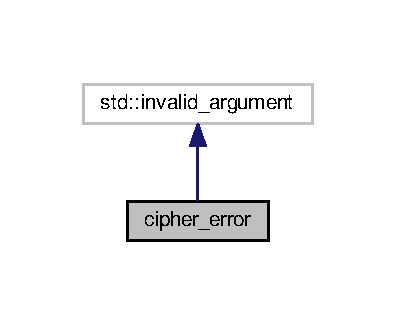
\includegraphics[width=190pt]{classcipher__error__inherit__graph}
\end{center}
\end{figure}


Граф связей класса cipher\+\_\+error\+:\nopagebreak
\begin{figure}[H]
\begin{center}
\leavevmode
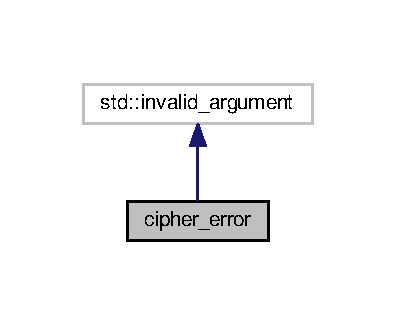
\includegraphics[width=190pt]{classcipher__error__coll__graph}
\end{center}
\end{figure}
\subsection*{Открытые члены}
\begin{DoxyCompactItemize}
\item 
{\bfseries cipher\+\_\+error} (const std\+::string \&what\+\_\+arg)\hypertarget{classcipher__error_aac662e216a84bfeb873303c7b88d029e}{}\label{classcipher__error_aac662e216a84bfeb873303c7b88d029e}

\item 
{\bfseries cipher\+\_\+error} (const char $\ast$what\+\_\+arg)\hypertarget{classcipher__error_a18cf27d9c2cd2538d3cb8f17e9a55f3e}{}\label{classcipher__error_a18cf27d9c2cd2538d3cb8f17e9a55f3e}

\end{DoxyCompactItemize}


Объявления и описания членов класса находятся в файле\+:\begin{DoxyCompactItemize}
\item 
\hyperlink{modAlphaCipher_8h}{mod\+Alpha\+Cipher.\+h}\end{DoxyCompactItemize}

\hypertarget{classPerestanovka}{}\section{Класс Perestanovka}
\label{classPerestanovka}\index{Perestanovka@{Perestanovka}}


Шифрование методом табличной маршрутной перестановки.  




{\ttfamily \#include $<$Perestanovka.\+h$>$}

\subsection*{Открытые члены}
\begin{DoxyCompactItemize}
\item 
\hyperlink{classPerestanovka_aa911a70c97003bd545ed52a4832c3d2b}{Perestanovka} ()=delete
\begin{DoxyCompactList}\small\item\em Конструктор без параметра. \end{DoxyCompactList}\item 
\hyperlink{classPerestanovka_a376d268a9c582ad2732d5013dc3ff08b}{Perestanovka} (const int \hyperlink{classPerestanovka_a7bd5d0e646ddcc4436dc058f505916c1}{k})
\begin{DoxyCompactList}\small\item\em Конструктор для установки ключа. \end{DoxyCompactList}\item 
std\+::string \hyperlink{classPerestanovka_a95ea7acda9a02a89903e4058a664fbcd}{shifr} (const std\+::string \&t)
\begin{DoxyCompactList}\small\item\em Метод для шифрования текста методом маршрутной табличной перестановки. \end{DoxyCompactList}\item 
std\+::string \hyperlink{classPerestanovka_ac0c30a5771b3de3c9bd2dde54cc93688}{rashifr} (const std\+::string \&z)
\begin{DoxyCompactList}\small\item\em Метод для расшифровки зашифрованного текста по известному ключу. \end{DoxyCompactList}\end{DoxyCompactItemize}
\subsection*{Закрытые члены}
\begin{DoxyCompactItemize}
\item 
std\+::string \hyperlink{classPerestanovka_a94bea2b10ae0897d6455ae6fd85994e7}{get\+Valid\+Open\+Text} (const std\+::string \&s)\hypertarget{classPerestanovka_a94bea2b10ae0897d6455ae6fd85994e7}{}\label{classPerestanovka_a94bea2b10ae0897d6455ae6fd85994e7}

\begin{DoxyCompactList}\small\item\em Метод проверки открытого текста. \end{DoxyCompactList}\item 
std\+::string \hyperlink{classPerestanovka_a990a3d3603a13242b16c2ba829405788}{get\+Valid\+Cipher\+Text} (const std\+::string \&s)\hypertarget{classPerestanovka_a990a3d3603a13242b16c2ba829405788}{}\label{classPerestanovka_a990a3d3603a13242b16c2ba829405788}

\begin{DoxyCompactList}\small\item\em Метод проверки зашифрованного текста. \end{DoxyCompactList}\end{DoxyCompactItemize}
\subsection*{Закрытые данные}
\begin{DoxyCompactItemize}
\item 
int \hyperlink{classPerestanovka_a7bd5d0e646ddcc4436dc058f505916c1}{k}\hypertarget{classPerestanovka_a7bd5d0e646ddcc4436dc058f505916c1}{}\label{classPerestanovka_a7bd5d0e646ddcc4436dc058f505916c1}

\begin{DoxyCompactList}\small\item\em Ключ \end{DoxyCompactList}\end{DoxyCompactItemize}


\subsection{Подробное описание}
Шифрование методом табличной маршрутной перестановки. 

Ключ устанавливается в конструкторе. Для зашифровывания и расшифровывания предназначены методы shifr и rashifr. \begin{DoxyWarning}{Предупреждения}
Реализация только для английского языка. 
\end{DoxyWarning}


\subsection{Конструктор(ы)}
\index{Perestanovka@{Perestanovka}!Perestanovka@{Perestanovka}}
\index{Perestanovka@{Perestanovka}!Perestanovka@{Perestanovka}}
\subsubsection[{\texorpdfstring{Perestanovka()=delete}{Perestanovka()=delete}}]{\setlength{\rightskip}{0pt plus 5cm}Perestanovka\+::\+Perestanovka (
\begin{DoxyParamCaption}
{}
\end{DoxyParamCaption}
)\hspace{0.3cm}{\ttfamily [delete]}}\hypertarget{classPerestanovka_aa911a70c97003bd545ed52a4832c3d2b}{}\label{classPerestanovka_aa911a70c97003bd545ed52a4832c3d2b}


Конструктор без параметра. 

Конструктор запрещён. \index{Perestanovka@{Perestanovka}!Perestanovka@{Perestanovka}}
\index{Perestanovka@{Perestanovka}!Perestanovka@{Perestanovka}}
\subsubsection[{\texorpdfstring{Perestanovka(const int k)}{Perestanovka(const int k)}}]{\setlength{\rightskip}{0pt plus 5cm}Perestanovka\+::\+Perestanovka (
\begin{DoxyParamCaption}
\item[{const int}]{k}
\end{DoxyParamCaption}
)}\hypertarget{classPerestanovka_a376d268a9c582ad2732d5013dc3ff08b}{}\label{classPerestanovka_a376d268a9c582ad2732d5013dc3ff08b}


Конструктор для установки ключа. 


\begin{DoxyParams}[1]{Аргументы}
\mbox{\tt in}  & {\em k} & -\/ ключ, целое, положительное число. \\
\hline
\end{DoxyParams}

\begin{DoxyExceptions}{Исключения}
{\em \hyperlink{classcipher__error}{cipher\+\_\+error},если} & ключ меньше или равен 1. \\
\hline
\end{DoxyExceptions}


\subsection{Методы}
\index{Perestanovka@{Perestanovka}!rashifr@{rashifr}}
\index{rashifr@{rashifr}!Perestanovka@{Perestanovka}}
\subsubsection[{\texorpdfstring{rashifr(const std\+::string \&z)}{rashifr(const std::string &z)}}]{\setlength{\rightskip}{0pt plus 5cm}std\+::string Perestanovka\+::rashifr (
\begin{DoxyParamCaption}
\item[{const std\+::string \&}]{z}
\end{DoxyParamCaption}
)}\hypertarget{classPerestanovka_ac0c30a5771b3de3c9bd2dde54cc93688}{}\label{classPerestanovka_ac0c30a5771b3de3c9bd2dde54cc93688}


Метод для расшифровки зашифрованного текста по известному ключу. 


\begin{DoxyParams}[1]{Аргументы}
\mbox{\tt in}  & {\em z} & Зашифрованный текст. Должен содержать только символы английского алфавита в верхнем регистре. Строка не должна быть пустой. \\
\hline
\end{DoxyParams}
\begin{DoxyReturn}{Возвращает}
Расшифрованный текст. 
\end{DoxyReturn}

\begin{DoxyExceptions}{Исключения}
{\em \hyperlink{classcipher__error}{cipher\+\_\+error},если} & строка пустая или встречена не английская буква в верхнем регистре. \\
\hline
\end{DoxyExceptions}
\index{Perestanovka@{Perestanovka}!shifr@{shifr}}
\index{shifr@{shifr}!Perestanovka@{Perestanovka}}
\subsubsection[{\texorpdfstring{shifr(const std\+::string \&t)}{shifr(const std::string &t)}}]{\setlength{\rightskip}{0pt plus 5cm}std\+::string Perestanovka\+::shifr (
\begin{DoxyParamCaption}
\item[{const std\+::string \&}]{t}
\end{DoxyParamCaption}
)}\hypertarget{classPerestanovka_a95ea7acda9a02a89903e4058a664fbcd}{}\label{classPerestanovka_a95ea7acda9a02a89903e4058a664fbcd}


Метод для шифрования текста методом маршрутной табличной перестановки. 

Запись в таблицу происходит слева направо, сверху вниз. Считывание из таблицы сверху вниз, справа налево 
\begin{DoxyParams}[1]{Аргументы}
\mbox{\tt in}  & {\em t} & Открытый текст. Не должен быть пустой строкой. Текст не должен быть меньше или равен длине ключа. Все не-\/буквы будут автоматически удалены. \\
\hline
\end{DoxyParams}
\begin{DoxyReturn}{Возвращает}
Зашифрованный текст. 
\end{DoxyReturn}

\begin{DoxyExceptions}{Исключения}
{\em \hyperlink{classcipher__error}{cipher\+\_\+error},если} & строка пустая или меньше или равна длине ключа. \\
\hline
\end{DoxyExceptions}


Объявления и описания членов классов находятся в файлах\+:\begin{DoxyCompactItemize}
\item 
\hyperlink{Perestanovka_8h}{Perestanovka.\+h}\item 
Perestanovka.\+cpp\end{DoxyCompactItemize}

\chapter{Файлы}
\hypertarget{Perestanovka_8h}{}\section{Файл Perestanovka.\+h}
\label{Perestanovka_8h}\index{Perestanovka.\+h@{Perestanovka.\+h}}


Заголовочный файл для модуля \hyperlink{classPerestanovka}{Perestanovka}.  


{\ttfamily \#include $<$string$>$}\\*
{\ttfamily \#include $<$stdexcept$>$}\\*
Граф включаемых заголовочных файлов для Perestanovka.\+h\+:\nopagebreak
\begin{figure}[H]
\begin{center}
\leavevmode
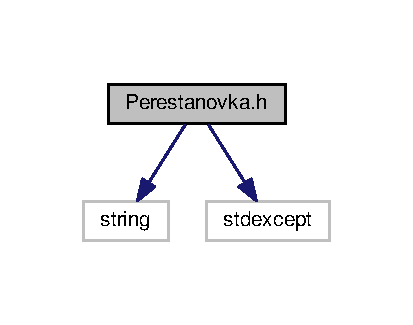
\includegraphics[width=198pt]{Perestanovka_8h__incl}
\end{center}
\end{figure}
\subsection*{Классы}
\begin{DoxyCompactItemize}
\item 
class \hyperlink{classPerestanovka}{Perestanovka}
\begin{DoxyCompactList}\small\item\em Шифрование методом табличной маршрутной перестановки. \end{DoxyCompactList}\item 
class \hyperlink{classcipher__error}{cipher\+\_\+error}
\end{DoxyCompactItemize}


\subsection{Подробное описание}
Заголовочный файл для модуля \hyperlink{classPerestanovka}{Perestanovka}. 

\begin{DoxyAuthor}{Автор}
Асаян А.\+В. 
\end{DoxyAuthor}
\begin{DoxyVersion}{Версия}
1.\+0 
\end{DoxyVersion}
\begin{DoxyDate}{Дата}
28.\+05.\+2019 
\end{DoxyDate}
\begin{DoxyCopyright}{Авторство}
ИБСТ ПГУ 
\end{DoxyCopyright}
\begin{DoxyWarning}{Предупреждения}
Работа студента. 
\end{DoxyWarning}

%--- End generated contents ---

% Index
\backmatter
\newpage
\phantomsection
\clearemptydoublepage
\addcontentsline{toc}{chapter}{Алфавитный указатель}
\printindex

\end{document}
